\documentclass[russian]{article}
\usepackage[T1]{fontenc}
\usepackage[utf8]{inputenc}
\usepackage{amssymb,esint,babel,qtree,ulem}
\usepackage{graphicx}
\makeatletter
\makeatother
\pagestyle{myheadings}
\markright{Александров А., 3372}

\begin{document}

\section*{2.1}

\paragraph*{а}

ищем кратчайшее ребро. если оно не образует цикл с выбранными ранее, добавляем его в дерево, иначе выбрасываем из таблицы.

\begin{tabular}{|c|c|c|c|c|c|c|c|}\hline
    & 1  & 2  & 3  & 4	& 5	 & 6  & 7\\\hline
1	& -- & {\bf 36} & 44 & {\bf 37} & 41 & 53 & 43\\\hline
2	&    & -- & 48 & 57 & 43 & 45 & 51\\\hline
3	&    &    & -- & 39 & 39 & {\bf 42} & {\bf 38}\\\hline
4	&    &    &    & -- & 52 & 51 & {\bf 34}\\\hline
5	&    &    &    &    & -- & 49 & {\bf 35}\\\hline
6	&    &    &    &    &    & -- & 45\\\hline
7	&    &    &    &    &    &    & -- \\\hline
\end{tabular}

\Tree [.4 7 ]

\Tree [.7 4 5 ]

\Tree [.7 4 5 ]
\Tree [.1 2 ]

\Tree [.4 [.7 5 ] [.1 2 ] ]

\Tree [.4 [.7 3 5 ] [.1 2 ] ]

выкидываем ребра (3,4), (3,5), (4,5), т.к. они образуют циклы

\Tree [.4 [.7 [.3 6 ] 5 ] [.1 2 ] ]

\paragraph*{б}

пусть полученное дерево $T_s$ неоптимально, а значит существует оптимальное дерево $T_o$. количество ребер $T_s$ и $T_o$ совпадает.
$E(T_s) = \{e_1, ..., e_{n-1}\}$, $w_i = w(e_i)$. $E(T_o) = \{e_1^*, ..., e_{n-1}^*\}$, $w_i* = w(e_i^*)$.
$w(T_s)=\sum_{i=1}^{n-1}w_i$, $w_i \ge w_j \forall i>j$. $w(T_o)=\sum_{i=1}^{n-1}w_i^*$, $w_i^* \ge w_j^* \forall i>j$.
$w(T_s) > w(T_o) \Rightarrow \exists min k : w_k > w_k^*$, но это невозможно, т.к. $w_k > w_{k-1}^* \ge ... $ .
в момент $k$ работы алгоритма найдется $k$ ребер, образующих лес и более легких, чем $e_k$. 
по лемме о пополнении леса в ${e_1^*, ..., e_k^*}$ существует ребро, не входящее в $\{e_1, ..., e_k\}$ и такое, что добавление его в $\{e_1, ..., e_k\}$ порождает лес $\Rightarrow$ противоречие.

\section*{2.2}

\paragraph*{а} алгоритм Дейкстры:

($\infty$, 0, $\infty$, $\infty$, $\infty$, $\infty$, $\infty$)

(56, \sout{0}, $\infty$, 54, $\infty$, $\infty$, 34)

(56, \sout{0}, $\infty$, 37, $\infty$, 77, \sout{34})

(56, \sout{0}, 42, \sout{37}, 76, 67, \sout{34})

(56, \sout{0}, \sout{42}, \sout{37}, 76, 67, \sout{34})

(\sout{56}, \sout{0}, \sout{42}, \sout{37}, 76, 67, \sout{34})

(\sout{56}, \sout{0}, \sout{42}, \sout{37}, 76, \sout{67}, \sout{34})

(\sout{56}, \sout{0}, \sout{42}, \sout{37}, \sout{76}, \sout{67}, \sout{34})

(56, 0, 42, 37, 76, 67, 34)

\paragraph*{б} доказательство корректности алгоритма Дейкстры:

пусть $l(v)$ — длина кратчайшего пути из вершины $a$ в вершину $v$. докажем по индукции, что в момент посещения любой вершины $z$, $d(z)=l(z)$.

база: первой посещается вершина $a$. в этот момент $d(a)=l(a)=0$.

шаг: пускай мы выбрали для посещения вершину $z \ne a$. докажем, что в этот момент $d(z)=l(z)$. для начала отметим, что для любой вершины $v$, всегда выполняется $d(v) \ge l(v)$ (алгоритм не может найти путь короче, чем кратчайший из всех существующих). пусть $P$ — кратчайший путь из $a$ в $z$, $y$ — первая непосещённая вершина на $P$, $x$ — предшествующая ей (следовательно, посещённая). поскольку путь $P$ кратчайший, его часть, ведущая из $a$ через $x$ в $y$, тоже кратчайшая, следовательно $l(y)=l(x)+w(xy)$. по предположению индукции, в момент посещения вершины $x$ выполнялось $d(x)=l(x)$, следовательно, вершина $y$ тогда получила метку не больше чем $d(x)+w(xy)=l(x)+w(xy)=l(y)$. следовательно, $d(y)=l(y)$. с другой стороны, поскольку сейчас мы выбрали вершину $z$, её метка минимальна среди непосещённых, то есть $d(z) \le d(y) = l(y) \le l(z)$. комбинируя это с $d(z) \ge l(z)$, имеем $d(z)=l(z)$, что и требовалось доказать.

поскольку алгоритм заканчивает работу, когда все вершины посещены, в этот момент $d=l$ для всех вершин.

\paragraph*{в} алгоритм Флойда-Уоршелла:

\begin{tabular}{|c|c|c|c|c|c|c|c|}\hline
& 1& 2& 3& 4& 5& 6& 7\\\hline
1&0&$\infty$&23&$\infty$&$\infty$&66&$\infty$\\\hline
2&56&0&$\infty$&54&$\infty$&$\infty$&34\\\hline
3&$\infty$&56&0&$\infty$&$\infty$&$\infty$&$\infty$\\\hline
4&$\infty$&$\infty$&5&0&39&30&$\infty$\\\hline
5&34&$\infty$&$\infty$&$\infty$&0&$\infty$&46\\\hline
6&$\infty$&$\infty$&73&31&19&0&4\\\hline
7&$\infty$&$\infty$&$\infty$&3&$\infty$&43&0\\\hline
\end{tabular}

\begin{tabular}{|c|c|c|c|c|c|c|c|}\hline
& 1& 2& 3& 4& 5& 6& 7\\\hline
1&0&$\infty$&23&$\infty$&$\infty$&66&$\infty$\\\hline
2&56&0&79&54&$\infty$&122&34\\\hline
3&$\infty$&56&0&$\infty$&$\infty$&$\infty$&$\infty$\\\hline
4&$\infty$&$\infty$&5&0&39&30&$\infty$\\\hline
5&34&$\infty$&57&$\infty$&0&100&46\\\hline
6&$\infty$&$\infty$&73&31&19&0&4\\\hline
7&$\infty$&$\infty$&$\infty$&3&$\infty$&43&0\\\hline
\end{tabular}

\begin{tabular}{|c|c|c|c|c|c|c|c|}\hline
& 1& 2& 3& 4& 5& 6& 7\\\hline
1&0&$\infty$&23&$\infty$&$\infty$&66&$\infty$\\\hline
2&56&0&79&54&$\infty$&122&34\\\hline
3&112&56&0&110&$\infty$&178&90\\\hline
4&$\infty$&$\infty$&5&0&39&30&$\infty$\\\hline
5&34&$\infty$&57&$\infty$&0&100&46\\\hline
6&$\infty$&$\infty$&73&31&19&0&4\\\hline
7&$\infty$&$\infty$&$\infty$&3&$\infty$&43&0\\\hline
\end{tabular}

\begin{tabular}{|c|c|c|c|c|c|c|c|}\hline
& 1& 2& 3& 4& 5& 6& 7\\\hline
1&0&79&23&133&$\infty$&66&113\\\hline
2&56&0&79&54&$\infty$&122&34\\\hline
3&112&56&0&110&$\infty$&178&90\\\hline
4&117&61&5&0&39&30&95\\\hline
5&34&113&57&167&0&100&46\\\hline
6&185&129&73&31&19&0&4\\\hline
7&$\infty$&$\infty$&$\infty$&3&$\infty$&43&0\\\hline
\end{tabular}

\begin{tabular}{|c|c|c|c|c|c|c|c|}\hline
& 1& 2& 3& 4& 5& 6& 7\\\hline
1&0&79&23&133&172&66&113\\\hline
2&56&0&59&54&93&84&34\\\hline
3&112&56&0&110&149&140&90\\\hline
4&117&61&5&0&39&30&95\\\hline
5&34&113&57&167&0&100&46\\\hline
6&148&92&36&31&19&0&4\\\hline
7&120&64&8&3&42&33&0\\\hline
\end{tabular}

\begin{tabular}{|c|c|c|c|c|c|c|c|}\hline
& 1& 2& 3& 4& 5& 6& 7\\\hline
1&0&79&23&133&172&66&113\\\hline
2&56&0&59&54&93&84&34\\\hline
3&112&56&0&110&149&140&90\\\hline
4&73&61&5&0&39&30&85\\\hline
5&34&113&57&167&0&100&46\\\hline
6&53&92&36&31&19&0&4\\\hline
7&76&64&8&3&42&33&0\\\hline
\end{tabular}

\begin{tabular}{|c|c|c|c|c|c|c|c|}\hline
& 1& 2& 3& 4& 5& 6& 7\\\hline
1&0&79&23&97&85&66&70\\\hline
2&56&0&59&54&93&84&34\\\hline
3&112&56&0&110&149&140&90\\\hline
4&73&61&5&0&39&30&34\\\hline
5&34&113&57&131&0&100&46\\\hline
6&53&92&36&31&19&0&4\\\hline
7&76&64&8&3&42&33&0\\\hline
\end{tabular}

\begin{tabular}{|c|c|c|c|c|c|c|c|}\hline
& 1& 2& 3& 4& 5& 6& 7\\\hline
1&0&79&23&73&85&66&70\\\hline
2&56&0&42&37&76&67&34\\\hline
3&112&56&0&93&132&123&90\\\hline
4&73&61&5&0&39&30&34\\\hline
5&34&110&54&49&0&79&46\\\hline
6&53&68&12&7&19&0&4\\\hline
7&76&64&8&3&42&33&0\\\hline
\end{tabular}

\paragraph*{г} доказательство корректности:

по индукции

база: $d_0(i,j)=w_{i,j}$

шаг: если кратчайшее расстояние от $i$ до $j$ через $\{1, ..., k+1\}$ не проходит через $k+1$, то верно

иначе $min(d_k(i, k+1), d_k(k+1, j)) \le d_k(i, j) \Rightarrow d_{k+1}(i,j)$ - искомое для этого шага

\section*{2.3}

\paragraph*{а}

\begin{tabular}{|c|c|c|c|c|c|c|c|}\hline
& 1& 2& 3& 4& 5& 6& 7\\\hline
1&0&0&23&0&0&66&0\\\hline
2&56&0&0&54&0&0&34\\\hline
3&0&56&0&0&0&0&0\\\hline
4&0&0&5&0&39&30&0\\\hline
5&34&0&0&0&0&0&46\\\hline
6&0&0&73&31&19&0&4\\\hline
7&0&0&0&3&0&43&0\\\hline
\end{tabular}

$ 2 \to 1 \to 6 \to 3 : 56$

\begin{tabular}{|c|c|c|c|c|c|c|c|}\hline
& 1& 2& 3& 4& 5& 6& 7\\\hline
1&0&56&23&0&0&10&0\\\hline
2&0&0&0&54&0&0&34\\\hline
3&0&56&0&0&0&56&0\\\hline
4&0&0&5&0&39&30&0\\\hline
5&34&0&0&0&0&0&46\\\hline
6&56&0&17&31&19&0&4\\\hline
7&0&0&0&3&0&43&0\\\hline
\end{tabular}

$ 2 \to 4 \to 5 \to 1 \to 3 : 23$

\begin{tabular}{|c|c|c|c|c|c|c|c|}\hline
& 1& 2& 3& 4& 5& 6& 7\\\hline
1&0&56&0&0&23&10&0\\\hline
2&0&0&0&31&0&0&34\\\hline
3&23&56&0&0&0&56&0\\\hline
4&0&23&5&0&16&30&0\\\hline
5&11&0&0&23&0&0&46\\\hline
6&56&0&17&31&19&0&4\\\hline
7&0&0&0&3&0&43&0\\\hline
\end{tabular}

$ 2 \to 4 \to 6 \to 3 : 17$

\begin{tabular}{|c|c|c|c|c|c|c|c|}\hline
& 1& 2& 3& 4& 5& 6& 7\\\hline
1&0&56&0&0&23&10&0\\\hline
2&0&0&0&14&0&0&34\\\hline
3&23&56&0&0&0&73&0\\\hline
4&0&40&5&0&16&13&0\\\hline
5&11&0&0&23&0&0&46\\\hline
6&56&0&0&48&19&0&4\\\hline
7&0&0&0&3&0&43&0\\\hline
\end{tabular}

$ 2 \to 4 \to 3 : 5$

\begin{tabular}{|c|c|c|c|c|c|c|c|}\hline
& 1& 2& 3& 4& 5& 6& 7\\\hline
1&0&56&0&0&23&10&0\\\hline
2&0&0&0&9&0&0&34\\\hline
3&23&56&0&5&0&73&0\\\hline
4&0&45&0&0&16&13&0\\\hline
5&11&0&0&23&0&0&46\\\hline
6&56&0&0&48&19&0&4\\\hline
7&0&0&0&3&0&43&0\\\hline
\end{tabular}

$M_f=56+23+17+5=101$

\paragraph*{б}

рассмотрим следующую сеть ($1 \to 4$), пропускная способность которой, очевидно, равна 2:

\begin{tabular}{|c|c|c|c|c|}\hline
& 1& 2& 3& 4\\\hline
1&0&1&1&0\\\hline
2&0&0&1&1\\\hline
3&0&0&0&1\\\hline
4&0&0&0&0\\\hline
\end{tabular}

в качестве первого пути выберем $ 1 \to 2 \to 3 \to 4 : 1$

без увеличения пропускной способности обратных дуг это привело бы к неоптимальному результату:

\begin{tabular}{|c|c|c|c|c|}\hline
& 1& 2& 3& 4\\\hline
1&0&0&1&0\\\hline
2&0&0&0&1\\\hline
3&0&0&0&0\\\hline
4&0&0&0&0\\\hline
\end{tabular}

при этом, увеличив пропускную способность можно добиться максимума:

\begin{tabular}{|c|c|c|c|c|}\hline
& 1& 2& 3& 4\\\hline
1&0&0&1&0\\\hline
2&1&0&0&1\\\hline
3&0&1&0&0\\\hline
4&0&0&1&0\\\hline
\end{tabular}

$1 \to 3 \to 2 \to 4 : 1$

\begin{tabular}{|c|c|c|c|c|}\hline
& 1& 2& 3& 4\\\hline
1&0&0&0&0\\\hline
2&1&0&1&0\\\hline
3&1&0&0&0\\\hline
4&0&1&1&0\\\hline
\end{tabular}

\section*{2.4}

\paragraph*{а}

\begin{tabular}{|c|c|c|c|c|c|c|}\hline
& 1& 2& 3& 4& 5& 6\\\hline
1& $0$& $\frac{1}{5}$& $\frac{1}{4}$& $\frac{1}{3}$& $\frac{1}{2}$& $1$\\\hline
2& $\frac{1}{12}$& $0$& $\frac{1}{8}$& $\frac{1}{6}$& $\frac{1}{4}$& $\frac{1}{2}$\\\hline
3& $\frac{1}{18}$& $\frac{1}{15}$& $0$& $\frac{1}{9}$& $\frac{1}{6}$& $\frac{1}{3}$\\\hline
4& $\frac{1}{24}$& $\frac{1}{20}$& $\frac{1}{16}$& $0$& $\frac{1}{8}$& $\frac{1}{4}$\\\hline
5& $\frac{1}{30}$& $\frac{1}{25}$& $\frac{1}{20}$& $\frac{1}{15}$& $0$& $\frac{1}{5}$\\\hline
6& $\frac{1}{36}$& $\frac{1}{30}$& $\frac{1}{24}$& $\frac{1}{18}$& $\frac{1}{12}$& $0$\\\hline
\end{tabular}

$ 1 \to 6 : 1$

\begin{tabular}{|c|c|c|c|c|c|c|}\hline
& 1& 2& 3& 4& 5& 6\\\hline
1& $0$& $\frac{1}{5}$& $\frac{1}{4}$& $\frac{1}{3}$& $\frac{1}{2}$& $0$\\\hline
2& $\frac{1}{12}$& $0$& $\frac{1}{8}$& $\frac{1}{6}$& $\frac{1}{4}$& $\frac{1}{2}$\\\hline
3& $\frac{1}{18}$& $\frac{1}{15}$& $0$& $\frac{1}{9}$& $\frac{1}{6}$& $\frac{1}{3}$\\\hline
4& $\frac{1}{24}$& $\frac{1}{20}$& $\frac{1}{16}$& $0$& $\frac{1}{8}$& $\frac{1}{4}$\\\hline
5& $\frac{1}{30}$& $\frac{1}{25}$& $\frac{1}{20}$& $\frac{1}{15}$& $0$& $\frac{1}{5}$\\\hline
6& $\frac{37}{36}$& $\frac{1}{30}$& $\frac{1}{24}$& $\frac{1}{18}$& $\frac{1}{12}$& $0$\\\hline
\end{tabular}

$ 1 \to 3 \to 6 : \frac{1}{4}$

\begin{tabular}{|c|c|c|c|c|c|c|}\hline
& 1& 2& 3& 4& 5& 6\\\hline
1& $0$& $\frac{1}{5}$& $0$& $\frac{1}{3}$& $\frac{1}{2}$& $0$\\\hline
2& $\frac{1}{12}$& $0$& $\frac{1}{8}$& $\frac{1}{6}$& $\frac{1}{4}$& $\frac{1}{2}$\\\hline
3& $\frac{11}{36}$& $\frac{1}{15}$& $0$& $\frac{1}{9}$& $\frac{1}{6}$& $\frac{1}{12}$\\\hline
4& $\frac{1}{24}$& $\frac{1}{20}$& $\frac{1}{16}$& $0$& $\frac{1}{8}$& $\frac{1}{4}$\\\hline
5& $\frac{1}{30}$& $\frac{1}{25}$& $\frac{1}{20}$& $\frac{1}{15}$& $0$& $\frac{1}{5}$\\\hline
6& $\frac{37}{36}$& $\frac{1}{30}$& $\frac{7}{24}$& $\frac{1}{18}$& $\frac{1}{12}$& $0$\\\hline
\end{tabular}

$ 1 \to 4 \to 6 : \frac{1}{4}$

\begin{tabular}{|c|c|c|c|c|c|c|}\hline
& 1& 2& 3& 4& 5& 6\\\hline
1& $0$& $\frac{1}{5}$& $0$& $\frac{1}{12}$& $\frac{1}{2}$& $0$\\\hline
2& $\frac{1}{12}$& $0$& $\frac{1}{8}$& $\frac{1}{6}$& $\frac{1}{4}$& $\frac{1}{2}$\\\hline
3& $\frac{11}{36}$& $\frac{1}{15}$& $0$& $\frac{1}{9}$& $\frac{1}{6}$& $\frac{1}{12}$\\\hline
4& $\frac{7}{24}$& $\frac{1}{20}$& $\frac{1}{16}$& $0$& $\frac{1}{8}$& $0$\\\hline
5& $\frac{1}{30}$& $\frac{1}{25}$& $\frac{1}{20}$& $\frac{1}{15}$& $0$& $\frac{1}{5}$\\\hline
6& $\frac{37}{36}$& $\frac{1}{30}$& $\frac{7}{24}$& $\frac{11}{36}$& $\frac{1}{12}$& $0$\\\hline
\end{tabular}

$ 1 \to 2 \to 6 : \frac{1}{5}$

\begin{tabular}{|c|c|c|c|c|c|c|}\hline
& 1& 2& 3& 4& 5& 6\\\hline
1& $0$& $0$& $0$& $\frac{1}{12}$& $\frac{1}{2}$& $0$\\\hline
2& $\frac{17}{60}$& $0$& $\frac{1}{8}$& $\frac{1}{6}$& $\frac{1}{4}$& $\frac{3}{10}$\\\hline
3& $\frac{11}{36}$& $\frac{1}{15}$& $0$& $\frac{1}{9}$& $\frac{1}{6}$& $\frac{1}{12}$\\\hline
4& $\frac{7}{24}$& $\frac{1}{20}$& $\frac{1}{16}$& $0$& $\frac{1}{8}$& $0$\\\hline
5& $\frac{1}{30}$& $\frac{1}{25}$& $\frac{1}{20}$& $\frac{1}{15}$& $0$& $\frac{1}{5}$\\\hline
6& $\frac{37}{36}$& $\frac{7}{30}$& $\frac{7}{24}$& $\frac{11}{36}$& $\frac{1}{12}$& $0$\\\hline
\end{tabular}

$ 1 \to 5 \to 6 : \frac{1}{5}$

\begin{tabular}{|c|c|c|c|c|c|c|}\hline
& 1& 2& 3& 4& 5& 6\\\hline
1& $0$& $0$& $0$& $\frac{1}{12}$& $\frac{3}{10}$& $0$\\\hline
2& $\frac{17}{60}$& $0$& $\frac{1}{8}$& $\frac{1}{6}$& $\frac{1}{4}$& $\frac{3}{10}$\\\hline
3& $\frac{11}{36}$& $\frac{1}{15}$& $0$& $\frac{1}{9}$& $\frac{1}{6}$& $\frac{1}{12}$\\\hline
4& $\frac{7}{24}$& $\frac{1}{20}$& $\frac{1}{16}$& $0$& $\frac{1}{8}$& $0$\\\hline
5& $\frac{7}{30}$& $\frac{1}{25}$& $\frac{1}{20}$& $\frac{1}{15}$& $0$& $0$\\\hline
6& $\frac{37}{36}$& $\frac{7}{30}$& $\frac{7}{24}$& $\frac{11}{36}$& $\frac{17}{60}$& $0$\\\hline
\end{tabular}

$ 1 \to 4 \to 3 \to 6 : \frac{1}{16}$

\begin{tabular}{|c|c|c|c|c|c|c|}\hline
& 1& 2& 3& 4& 5& 6\\\hline
1& $0$& $0$& $0$& $\frac{1}{48}$& $\frac{3}{10}$& $0$\\\hline
2& $\frac{17}{60}$& $0$& $\frac{1}{8}$& $\frac{1}{6}$& $\frac{1}{4}$& $\frac{3}{10}$\\\hline
3& $\frac{11}{36}$& $\frac{1}{15}$& $0$& $\frac{25}{144}$& $\frac{1}{6}$& $\frac{1}{48}$\\\hline
4& $\frac{17}{48}$& $\frac{1}{20}$& $0$& $0$& $\frac{1}{8}$& $0$\\\hline
5& $\frac{7}{30}$& $\frac{1}{25}$& $\frac{1}{20}$& $\frac{1}{15}$& $0$& $0$\\\hline
6& $\frac{37}{36}$& $\frac{7}{30}$& $\frac{17}{48}$& $\frac{11}{36}$& $\frac{17}{60}$& $0$\\\hline
\end{tabular}

$ 1 \to 5 \to 3 \to 2 \to 6 : \frac{1}{20}$

\begin{tabular}{|c|c|c|c|c|c|c|}\hline
& 1& 2& 3& 4& 5& 6\\\hline
1& $0$& $0$& $0$& $\frac{1}{48}$& $\frac{1}{4}$& $0$\\\hline
2& $\frac{17}{60}$& $0$& $\frac{7}{40}$& $\frac{1}{6}$& $\frac{1}{4}$& $\frac{1}{4}$\\\hline
3& $\frac{11}{36}$& $\frac{1}{60}$& $0$& $\frac{25}{144}$& $\frac{13}{60}$& $\frac{1}{48}$\\\hline
4& $\frac{17}{48}$& $\frac{1}{20}$& $0$& $0$& $\frac{1}{8}$& $0$\\\hline
5& $\frac{17}{60}$& $\frac{1}{25}$& $0$& $\frac{1}{15}$& $0$& $0$\\\hline
6& $\frac{37}{36}$& $\frac{17}{60}$& $\frac{17}{48}$& $\frac{11}{36}$& $\frac{17}{60}$& $0$\\\hline
\end{tabular}

$ 1 \to 5 \to 4 \to 2 \to 6 : \frac{1}{20}$

\begin{tabular}{|c|c|c|c|c|c|c|}\hline
& 1& 2& 3& 4& 5& 6\\\hline
1& $0$& $0$& $0$& $\frac{1}{48}$& $\frac{1}{5}$& $0$\\\hline
2& $\frac{17}{60}$& $0$& $\frac{7}{40}$& $\frac{13}{60}$& $\frac{1}{4}$& $\frac{1}{5}$\\\hline
3& $\frac{11}{36}$& $\frac{1}{60}$& $0$& $\frac{25}{144}$& $\frac{13}{60}$& $\frac{1}{48}$\\\hline
4& $\frac{17}{48}$& $0$& $0$& $0$& $\frac{7}{40}$& $0$\\\hline
5& $\frac{1}{3}$& $\frac{1}{25}$& $0$& $\frac{1}{60}$& $0$& $0$\\\hline
6& $\frac{37}{36}$& $\frac{1}{3}$& $\frac{17}{48}$& $\frac{11}{36}$& $\frac{17}{60}$& $0$\\\hline
\end{tabular}

$ 1 \to 5 \to 2 \to 6 : \frac{1}{25}$

\begin{tabular}{|c|c|c|c|c|c|c|}\hline
& 1& 2& 3& 4& 5& 6\\\hline
1& $0$& $0$& $0$& $\frac{1}{48}$& $\frac{4}{25}$& $0$\\\hline
2& $\frac{17}{60}$& $0$& $\frac{7}{40}$& $\frac{13}{60}$& $\frac{29}{100}$& $\frac{4}{25}$\\\hline
3& $\frac{11}{36}$& $\frac{1}{60}$& $0$& $\frac{25}{144}$& $\frac{13}{60}$& $\frac{1}{48}$\\\hline
4& $\frac{17}{48}$& $0$& $0$& $0$& $\frac{7}{40}$& $0$\\\hline
5& $\frac{28}{75}$& $0$& $0$& $\frac{1}{60}$& $0$& $0$\\\hline
6& $\frac{37}{36}$& $\frac{28}{75}$& $\frac{17}{48}$& $\frac{11}{36}$& $\frac{17}{60}$& $0$\\\hline
\end{tabular}

$M_f=1+\frac{1}{4}+\frac{1}{4}+\frac{1}{5}+\frac{1}{5}+\frac{1}{16}+\frac{1}{20}+\frac{1}{20}+\frac{1}{25}=\frac{841}{400}$

\paragraph*{б,в}

рассмотрим сеть с источником $s$, стоком $t$, пропускными способностями рёбер $e_1$, $e_2$ и $e_3$ соответственно $1$, $r=\frac{\sqrt{5}-1}{2}$ и $1$ и пропускной способностью всех остальных рёбер $42$.

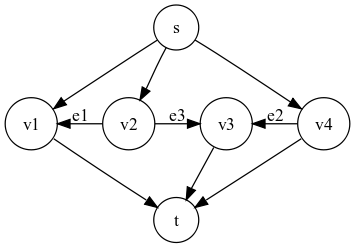
\includegraphics[scale=0.5]{dm_4_m2_4}

\begin{tabular}{|c|c|c|c|c|c|}\hline
шаг	& путь & поток & $e_1$	& $e_2$ & $e_3$ \\\hline
0	&&	& $r_0 = 1$ &	$r$ & 1 \\\hline
1	& $\{s,v_2,v_3,t\}$ &	1	&$r^0$ &	$r^1$ &	0 \\\hline
2	& $p_1=\{s,v_4,v_3,v_2,v_1,t\}$	& $r^1$	& $r^2$ &	0 &	$r^1$ \\\hline
3	& $p_2=\{s,v_2,v_3,v_4,t\}$	& $r^1$	& $r^2$&	$r^1$ &	0\\\hline
4	& $p_1$	& $r^2$	& 0	& $r^3$ &	$r^2$\\\hline
5	& $p_3=\{s,v_1,v_2,v_3\}$	& $r^2$	& $r^2$	& $r^3$ &	0\\\hline
\end{tabular}

после шага 1, как и после шага 5, остаточные способности рёбер $e_1$, $e_2$ и $e_3$ имеют форму $r^n$, $r^n + 1$ и $0$, соответственно. это значит, что можно использовать последовательность увеличивающих путей $\{p_1,p_2,p_1,p_3\}$ бесконечно много раз, и остаточные пропускные способности этих рёбер всегда будут в той же форме. полный поток после шага 5 равен $1 + 2(r^1 + r^2)$. за бесконечное время полный поток сойдётся к $1+2\sum_{i=1}^\infty r^i=3+2r=2+\sqrt{5}$, тогда как максимальный поток равен 85. т.е. при неоптимальном выборе увеличивающих путей АФФ на такой сети работает бесконечно долго и даже в пределе не достигает оптимального результата.

\section*{2.5}

\paragraph*{а} 

\begin{tabular}{|c|c|c|c|c|c|c|c|c|}\hline
& 1& 2& 3& 4& 5& 6& 7& $\alpha$\\\hline
1& & 36& 44& 37& 41& 53& 43& 36\\\hline
2& 42& & 48& 57& 43& 45& 51& 42\\\hline
3& 35& 41& & 39& 39& 42& 38& 35\\\hline
4& 38& 34& 35& & 52& 51& 34& 34\\\hline
5& 40& 43& 47& 37& & 49& 35& 35\\\hline
6& 33& 40& 56& 53& 36& & 45& 33\\\hline
7& 33& 39& 39& 36& 34& 48& & 33\\\hline
$\beta$& 0& 0& 1& 1& 1& 3& 0& 254\\\hline
\end{tabular}

проверяем 
$1 \to 2$

$1 \to 2 \to 5 \to 7 \to 4 \to 3 \to 6 \to 1$ : $H_{rec}$ = 260

\begin{tabular}{|c|c|c|c|c|c|c|c|c|}\hline
& 1& 2& 3& 4& 5& 6& 7& $\alpha$\\\hline
1& & 36& 44& 37& 41& 53& 43& 36\\\hline
2& 42& & 48& 57& 43& 45& 51& 42\\\hline
3& 35& 41& & 39& 39& 42& 38& 35\\\hline
4& 38& 34& 35& & 52& 51& 34& 34\\\hline
5& 40& 43& 47& 37& & 49& 35& 35\\\hline
6& 33& 40& 56& 53& 36& & 45& 33\\\hline
7& 33& 39& 39& 36& 34& 48& & 33\\\hline
$\beta$& 0& 0& 1& 1& 1& 3& 0& 254\\\hline
\end{tabular}

проверяем 
$1 \to 2 \to 3$

\begin{tabular}{|c|c|c|c|c|c|c|c|c|}\hline
& 1& 2& 3& 4& 5& 6& 7& $\alpha$\\\hline
1& & 36& & & & & & 36\\\hline
2& & & 48& & & & & 48\\\hline
3& & & & 39& 39& 42& 38& 38\\\hline
4& 38& & & & 52& 51& 34& 34\\\hline
5& 40& & & 37& & 49& 35& 35\\\hline
6& 33& & & 53& 36& & 45& 33\\\hline
7& 33& & & 36& 34& 48& & 33\\\hline
$\beta$& 0& 0& 0& 1& 1& 4& 0& 263\\\hline
\end{tabular}

$H_{min} > H_{rec} \Rightarrow $ отбрасываем дерево

проверяем 
$1 \to 2 \to 4$

\begin{tabular}{|c|c|c|c|c|c|c|c|c|}\hline
& 1& 2& 3& 4& 5& 6& 7& $\alpha$\\\hline
1& & 36& & & & & & 36\\\hline
2& & & & 57& & & & 57\\\hline
3& 35& & & & 39& 42& 38& 35\\\hline
4& & & 35& & 52& 51& 34& 34\\\hline
5& 40& & 47& & & 49& 35& 35\\\hline
6& 33& & 56& & 36& & 45& 33\\\hline
7& 33& & 39& & 34& 48& & 33\\\hline
$\beta$& 0& 0& 1& 0& 1& 7& 0& 272\\\hline
\end{tabular}

$H_{min} > H_{rec} \Rightarrow $ отбрасываем дерево

проверяем 
$1 \to 2 \to 5$

\begin{tabular}{|c|c|c|c|c|c|c|c|c|}\hline
& 1& 2& 3& 4& 5& 6& 7& $\alpha$\\\hline
1& & 36& & & & & & 36\\\hline
2& & & & & 43& & & 43\\\hline
3& 35& & & 39& & 42& 38& 35\\\hline
4& 38& & 35& & & 51& 34& 34\\\hline
5& & & 47& 37& & 49& 35& 35\\\hline
6& 33& & 56& 53& & & 45& 33\\\hline
7& 33& & 39& 36& & 48& & 33\\\hline
$\beta$& 0& 0& 1& 2& 0& 7& 0& 259\\\hline
\end{tabular}

проверяем 
$1 \to 2 \to 5 \to 3$

\begin{tabular}{|c|c|c|c|c|c|c|c|c|}\hline
& 1& 2& 3& 4& 5& 6& 7& $\alpha$\\\hline
1& & 36& & & & & & 36\\\hline
2& & & & & 43& & & 43\\\hline
3& & & & 39& & 42& 38& 38\\\hline
4& 38& & & & & 51& 34& 34\\\hline
5& & & 47& & & & & 47\\\hline
6& 33& & & 53& & & 45& 33\\\hline
7& 33& & & 36& & 48& & 33\\\hline
$\beta$& 0& 0& 0& 1& 0& 4& 0& 269\\\hline
\end{tabular}

$H_{min} > H_{rec} \Rightarrow $ отбрасываем дерево

проверяем 
$1 \to 2 \to 5 \to 4$

\begin{tabular}{|c|c|c|c|c|c|c|c|c|}\hline
& 1& 2& 3& 4& 5& 6& 7& $\alpha$\\\hline
1& & 36& & & & & & 36\\\hline
2& & & & & 43& & & 43\\\hline
3& 35& & & & & 42& 38& 35\\\hline
4& & & 35& & & 51& 34& 34\\\hline
5& & & & 37& & & & 37\\\hline
6& 33& & 56& & & & 45& 33\\\hline
7& 33& & 39& & & 48& & 33\\\hline
$\beta$& 0& 0& 1& 0& 0& 7& 0& 259\\\hline
\end{tabular}

проверяем 
$1 \to 2 \to 5 \to 4 \to 3$

\begin{tabular}{|c|c|c|c|c|c|c|c|c|}\hline
& 1& 2& 3& 4& 5& 6& 7& $\alpha$\\\hline
1& & 36& & & & & & 36\\\hline
2& & & & & 43& & & 43\\\hline
3& & & & & & 42& 38& 38\\\hline
4& & & 35& & & & & 35\\\hline
5& & & & 37& & & & 37\\\hline
6& 33& & & & & & 45& 33\\\hline
7& 33& & & & & 48& & 33\\\hline
$\beta$& 0& 0& 0& 0& 0& 4& 0& 259\\\hline
\end{tabular}

проверяем 
$1 \to 2 \to 5 \to 4 \to 3 \to 6$

\begin{tabular}{|c|c|c|c|c|c|c|c|c|}\hline
& 1& 2& 3& 4& 5& 6& 7& $\alpha$\\\hline
1& & 36& & & & & & 36\\\hline
2& & & & & 43& & & 43\\\hline
3& & & & & & 42& & 42\\\hline
4& & & 35& & & & & 35\\\hline
5& & & & 37& & & & 37\\\hline
6& & & & & & & 45& 45\\\hline
7& 33& & & & & & & 33\\\hline
$\beta$& 0& 0& 0& 0& 0& 0& 0& 271\\\hline
\end{tabular}

$H_{min} > H_{rec} \Rightarrow $ отбрасываем дерево

проверяем 
$1 \to 2 \to 5 \to 4 \to 3 \to 7$

\begin{tabular}{|c|c|c|c|c|c|c|c|c|}\hline
& 1& 2& 3& 4& 5& 6& 7& $\alpha$\\\hline
1& & 36& & & & & & 36\\\hline
2& & & & & 43& & & 43\\\hline
3& & & & & & & 38& 38\\\hline
4& & & 35& & & & & 35\\\hline
5& & & & 37& & & & 37\\\hline
6& 33& & & & & & & 33\\\hline
7& & & & & & 48& & 48\\\hline
$\beta$& 0& 0& 0& 0& 0& 0& 0& 270\\\hline
\end{tabular}

$H_{min} > H_{rec} \Rightarrow $ отбрасываем дерево

проверяем 
$1 \to 2 \to 5 \to 4 \to 6$

\begin{tabular}{|c|c|c|c|c|c|c|c|c|}\hline
& 1& 2& 3& 4& 5& 6& 7& $\alpha$\\\hline
1& & 36& & & & & & 36\\\hline
2& & & & & 43& & & 43\\\hline
3& 35& & & & & & 38& 35\\\hline
4& & & & & & 51& & 51\\\hline
5& & & & 37& & & & 37\\\hline
6& & & 56& & & & 45& 45\\\hline
7& 33& & 39& & & & & 33\\\hline
$\beta$& 0& 0& 6& 0& 0& 0& 0& 286\\\hline
\end{tabular}

$H_{min} > H_{rec} \Rightarrow $ отбрасываем дерево

проверяем 
$1 \to 2 \to 5 \to 4 \to 7$

\begin{tabular}{|c|c|c|c|c|c|c|c|c|}\hline
& 1& 2& 3& 4& 5& 6& 7& $\alpha$\\\hline
1& & 36& & & & & & 36\\\hline
2& & & & & 43& & & 43\\\hline
3& 35& & & & & 42& & 35\\\hline
4& & & & & & & 34& 34\\\hline
5& & & & 37& & & & 37\\\hline
6& 33& & 56& & & & & 33\\\hline
7& & & 39& & & 48& & 39\\\hline
$\beta$& 0& 0& 0& 0& 0& 7& 0& 264\\\hline
\end{tabular}

$H_{min} > H_{rec} \Rightarrow $ отбрасываем дерево

проверяем 
$1 \to 2 \to 5 \to 6$

\begin{tabular}{|c|c|c|c|c|c|c|c|c|}\hline
& 1& 2& 3& 4& 5& 6& 7& $\alpha$\\\hline
1& & 36& & & & & & 36\\\hline
2& & & & & 43& & & 43\\\hline
3& 35& & & 39& & & 38& 35\\\hline
4& 38& & 35& & & & 34& 34\\\hline
5& & & & & & 49& & 49\\\hline
6& & & 56& 53& & & 45& 45\\\hline
7& 33& & 39& 36& & & & 33\\\hline
$\beta$& 0& 0& 1& 3& 0& 0& 0& 279\\\hline
\end{tabular}

$H_{min} > H_{rec} \Rightarrow $ отбрасываем дерево

проверяем 
$1 \to 2 \to 5 \to 7$

\begin{tabular}{|c|c|c|c|c|c|c|c|c|}\hline
& 1& 2& 3& 4& 5& 6& 7& $\alpha$\\\hline
1& & 36& & & & & & 36\\\hline
2& & & & & 43& & & 43\\\hline
3& 35& & & 39& & 42& & 35\\\hline
4& 38& & 35& & & 51& & 35\\\hline
5& & & & & & & 35& 35\\\hline
6& 33& & 56& 53& & & & 33\\\hline
7& & & 39& 36& & 48& & 36\\\hline
$\beta$& 0& 0& 0& 0& 0& 7& 0& 260\\\hline
\end{tabular}

$H_{min} = H_{rec} \Rightarrow $ решение найдено:

$1 \to 2 \to 5 \to 7 \to 4 \to 3 \to 6 \to 1$

\paragraph*{б}

сначала жадным алгоритмом находим короткий цикл и называем его $H_{rec}$. далее находим $\alpha_i = \min_k c_{i,k}$ и $\beta_j=\min_k(c_{j,k}-\alpha_k)$. их сумма $H_{min}=\sum(\alpha_i+\beta_i)$ - нижняя оценка.
дальше рекурсивно обходим дерево вариантов. если $H_{min}=H_{rec}$, значит $H_{rec}$ - минимальный цикл. если $H_{min}>H_{rec}$, то в этом поддереве решений нет и его можно дальше не рассматривать.

\section*{2.7}

\paragraph*{а}

чтобы из $(0,...,0)$ получить $k$-элементное подмножество нужно преобразовать $k$ нулей в единицы. сделать это можно $n!$ способами. затем из $n!$ слоя нужно дойти до вершины. это еще $(n-k)!$ преобразований. и того $n!(n-k)!$ цепей. 

\paragraph*{б}

каждый слой это антицепь. $i$ - из $c_n^i$ элементов. антицепь из $c_n^{\lfloor\frac{n}{2}\rfloor}$ элементов - средний слой в диаграмме. те вершины в булевой решетке, в которых по $\lfloor\frac{n}{2}\rfloor$ единиц.

\paragraph*{в}

числа $C_n^{[\frac{n}{2}]}=\max_k C_n^k$, это максимальная мощность антицепи уровня $[\frac{n}{2}]$, по крайней мере мощность этой антицепи больше мощности антицепей на других уровнях $\Rightarrow$ разбиваем:

1) взять элемент на уровне $[\frac{n}{2}]$

2) убрать из одной из позиций 1

3) если попали в элемент, задействованный в одной из цепей, то убираем с другой, вернув первую

4) если перебрали все единицы и не выбрали элемент, то выбираем любой

5) записываем текущий элемент и проделываем для него шаг 1 пока не дойдем до 0

6) аналогично идем в сторону увеличения : возвращаемся к выбранному на $[\frac{n}{2}]$ уровне элементу

7) добавим 1 на одну из нулевых позиций

8) если попали в уже задействованный в одной из цепей элемент, то выбираем другую позицию

9) если не смогли выбрать - берем любую

10) заменяем текущий элемент и проделываем для него шаг 6, пока не дойдем до 1

11) берем следующий элемент на уровне $[\frac{n}{2}]$ и повторяем для него все то же самое, и так для всех $[\frac{n}{2}]$ элементов

$\Rightarrow $ получаем разбиение на $[\frac{n}{2}]$ цепей
\paragraph*{г}

следствие теоремы Дилворта (для любого частично упорядоченного множества $P = (S, \le)$ минимальное число цепей, покрывающих все точки $S$, равно мощности наибольшей антицепи, т.е., мощности множества несравнимых точек в $P$).

есть антицепи длины $C_n^1$, $C_n^2$, ..., $C_n^{n-1}$. рассмотрим монотонные функции, которые при $k-1$ аргументах равных 1 дают 0, а при $k+1$ - 1. при этом т.к. элементы с $k$ единицами образуют антицепь, монотонная функция на эти элементах может быть и 0 и 1.

таких элементов $C_n^k \Rightarrow $ таких функций $2^{C_n^k} \Rightarrow $ всего монотонных функций не менне, чем $\sum _{k=1}^{n-1} 2^{C_n^k}$

\end{document} 